% Single Labels. Slides 12 to 16. Each result follows its model explanation.
\section{Single Labels}

% Source. Methods 4.3.1 and 4.3.5, eq:ebnn-hierarchy, eq:ebnn-categorical,
% sec:ebnn-uncertainty-decomposition.
% Delivery. Identify w, alpha(x;w), and pi before discussing the label.
\begin{frame}{A Dirichlet network with a weight posterior}
\label{frm:cat-ebnn}
\slidemessage{The combined model represents the three uncertainty terms.}
\begin{itemize}
\item Categorical evidential Bayesian neural network (Cat-eBNN)
\begin{itemize}
\item For input $x$ and data $D$, the weight posterior $p(w\mid D)$ gives epistemic uncertainty.
\end{itemize}
\end{itemize}
\[
p(\pi\mid x,w)=\mathrm{Dir}\bigl(\pi\mid\alpha(x;w)\bigr)
\qquad \text{distributional uncertainty}
\]
\[
p(y\mid\pi)=\mathrm{Cat}(y\mid\pi)
\qquad \text{aleatoric uncertainty}
\]
\slidepoint{The network gives $\alpha(x;w)$. The random class-probability vector is $\pi$.}
% Copied from thesis eq:ebnn-hierarchy and eq:ebnn-categorical.
% Preparation. $x$ is the input, $D$ the observed dataset, and $w$ the shared network weights. The network produces $\alpha(x;w)$.
% Source detail. Thesis \S4.3.1 and \S4.3.5.
\end{frame}

% Source. Methods 4.3.2 and 4.3.3, eq:ebnn-likelihood-equivalence,
% eq:ebnn-likelihood-invariance. Background 2.3, eq:scale-invariance.
% Delivery. Keep the mean fixed. A change in concentration then leaves the likelihood unchanged.
\begin{frame}{The single label likelihood}
\label{frm:likelihood-limit}
\slidemessage{At fixed mean vectors, single labels cannot inform the total concentration parameter.}
% Copied from thesis eq:ebnn-likelihood-equivalence and eq:edl-predictive.
\[
p(y\mid x,w)=m_y(x;w),
\qquad m(x;w)=\frac{\alpha(x;w)}{\alpha_0(x;w)}.
\]
\medskip
% Thesis eq:scale-invariance. Generic Dirichlet vector and scalar, not network functions.
\[
\frac{\lambda\alpha}{\lambda\alpha_0}
=\frac{\alpha}{\alpha_0}=m,
\qquad \lambda>0.
\]
\medskip
\slidepoint{Rescaling changes total concentration without changing the mean vector or label likelihood.}
% Preparation. The identity concerns rescaled Dirichlet parameters. The network result compares weights with equal mean vectors on the training inputs.
% Source detail. Thesis \S2.3, \S4.3.2, and \S4.3.3.
\end{frame}

% Source. Methods 4.3.1 and 4.3.4, eq:gamma-prior-weights,
% eq:assumed-total-concentration. Background 2.10, eq:gamma-mode.
% Delivery. The Gamma factors act on network outputs, not on a new sampled variable.
\begin{frame}{An explicit Gamma prior}
\label{frm:gamma-prior}
\slidepoint{{\large The Gamma prior states an assumption about the\par total concentration parameter.}}
\begin{center}
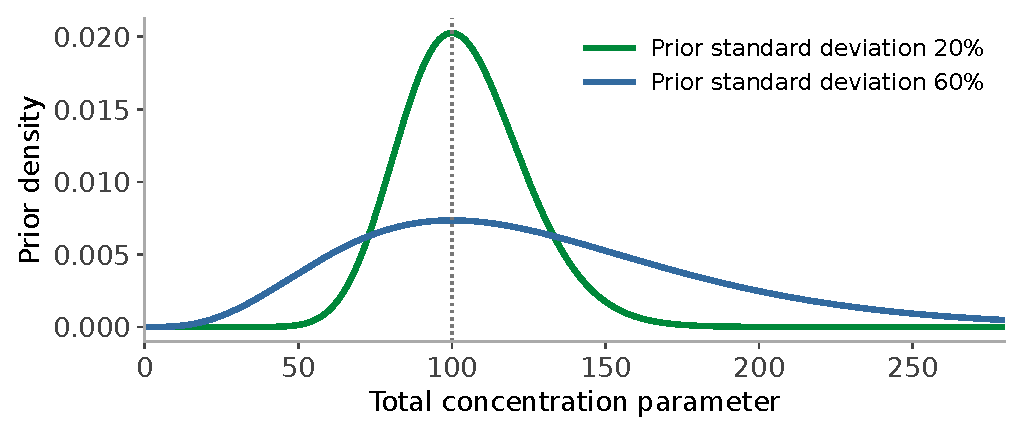
\includegraphics[width=0.70\textwidth]{figures/gamma_prior.pdf}
\end{center}
\begin{itemize}
\item Gamma factors act on network outputs at the training inputs.
\item Illustrative prior mode 100.
\begin{itemize}
\item Standard deviations are relative to this mode.
\end{itemize}
\end{itemize}
% Preparation. Illustrative prior mode 100. Standard deviations are relative to this mode.\par
% The prior acts on network outputs at the training inputs.
% Source detail. Thesis \S4.3.1 and \S4.3.4. Gamma factors are evaluated at the $N$ training inputs.
\end{frame}

% Source. Experiments 5.2.2, tab:e2-mode-sweep, eq:realised-total-concentration.
% Delivery. Read the prior mode, realised value, and direction of the shares. Do not read every number.
\begin{frame}{The prior changes the reported allocation}
\label{frm:prior-mode-results}
\slidemessage{Higher prior modes correspond to a lower distributional share in these runs.}
\begin{center}
\small
\renewcommand{\arraystretch}{1.5}
\setlength{\tabcolsep}{7pt}
% Generated by scripts/build_figures.py from unchanged thesis analysis outputs.
\begin{tabular}{cccc}
\toprule
\shortstack{Gamma prior\\mode} & \shortstack{realised total\\concentration} & \shortstack{aleatoric\\uncertainty \%} & \shortstack{distributional\\uncertainty \%} \\
\midrule
30 & 30.4\,(30.2--30.5) & 89.24 & 8.98 \\
100 & 99.7\,(99.5--99.8) & 91.11 & 4.79 \\
300 & 291.4\,(291.2--291.6) & 98.07 & 0.87 \\
\bottomrule
\end{tabular}

\end{center}
\begin{itemize}
\item The trained mean vectors also change across runs.
\item CIFAR-10. Means and ranges over three seeds.
\begin{itemize}
\item Final Bayesian model averaging (BMA) over ten samples.
\end{itemize}
\end{itemize}
% Preparation. CIFAR-10, ResNet-20. Final Bayesian model averaging (BMA) over ten samples.\par
% Three seeds. Prior standard deviation 20\%. Mode 30 uses warm initialisation. Higher modes use shifted initialisation.\par
% Parentheses show the seed range. Shares are percentages of average predictive uncertainty.
% Source detail. Thesis \S5.2.2.
\end{frame}

% Source. Experiments 5.2.4, tab:e2-predictive. Results keep the thesis precision.
% Delivery. State the absence of a consistent predictive gain, then return to the likelihood limitation.
\begin{frame}{Prediction with single labels}
\label{frm:single-prediction}
\slidemessage{Negative log likelihood favours the Cat-BNN on both datasets.}
\begin{itemize}
\item Negative log likelihood (NLL).
\begin{itemize}
\item Lower is better.
\end{itemize}
\item Accuracy results are mixed.
\end{itemize}
\begin{center}
\small
\renewcommand{\arraystretch}{1.22}
% Generated by scripts/build_figures.py from unchanged thesis analysis outputs.
\begin{tabular}{lcc}
\toprule
model & accuracy & NLL \\
\midrule
\multicolumn{3}{l}{\textbf{Fashion-MNIST}} \\
Cat-BNN & 0.921\,(0.917--0.924) & 0.221\,(0.211--0.230) \\
Cat-eBNN & 0.913\,(0.908--0.916) & 0.431\,(0.410--0.458) \\
\midrule
\multicolumn{3}{l}{\textbf{CIFAR-10}} \\
Cat-BNN & 0.856\,(0.850--0.859) & 0.426\,(0.418--0.441) \\
Cat-eBNN & 0.867\,(0.866--0.868) & 0.470\,(0.461--0.476) \\
\bottomrule
\end{tabular}

\end{center}
\par\medskip
\slidepoint{Means and ranges over three seeds. Final BMA over ten samples.}
% Preparation. Mean and range over three seeds. Final BMA over ten samples.\par
% Cat-BNN uses warm initialisation. Cat-eBNN uses shifted initialisation, prior mode 100, and prior standard deviation 20\%.
% Source detail. Thesis \S5.2.4.
\end{frame}
